% !TEX root =  ../unref_general.tex
%\section{Indicators for non-SPD problems}
\section{Model problem}
\label{sec:Model-problem}
%\subsection{Laplace Goal-Oriented Problem}
%Let us consider the following Laplace Goal-Oriented problem.
%\begin{var_for}
%	Find $u$ such that,
%	\begin{equation}
%		\begin{cases}
%			- \Delta u= \mathds{1}_{(0,0.25)^{2}} &\text{ in } \Omega,\\
%			u=0 & \text{ on } {\partial \Omega=\Gamma_{D}},\\
%		\end{cases}
%	\end{equation}
%\end{var_for}
%\noindent with $\Omega\subset \R^{d}$ a domain, $d$=2 or 3  its spatial dimension, $\H$ an Hilbert space on $\Omega$, and $\Omega=(0,1)^{2}\symbol{92} (\frac{1}{2},1) \times (0,\frac{1}{2})$. We denote the boundary of $\Omega$ as $\partial \Omega \coloneqq \Gamma_{D}$. We define the \ac{QoI} as $l(\phi)=\int_{\Omega} \mathds{1}_{(0.75,1)^{2}}\phi$, $\forall \phi \in \H$. \Cref{fig:LaplaceGOA} illustrates the computational domain.
%
%\begin{figure}
%	\begin{tikzpicture}[x=2.5cm,y=2.5cm]
%		\node(n1) at (0,0){};
%		\node(n2) at (1,0){};
%		\node(n3) at (1,1){};
%		\node(n4) at (0,1){};
%
%		\node(n5) at (0.25,0.25){};
%		\node(n6) at (0.75,0.25){};
%		\node(n7) at (0.75,0.75){};
%		\node(n8) at (0.5,0.5){};
%
%		\draw[color=blue, thick] (n4.center) --  (n3.center) -- node[pos=0.25,pin={0: $\Gamma_{D}$}]{} (n2.center);
%
%		\draw[color=blue, thick,] (n1) rectangle (n3);
%		\draw[color=blue, thick, fill=gray] (n2) rectangle (n8);
%
%		\draw (n1) rectangle (n5) node[pos=0.5] {$f$};
%		\draw (n7) rectangle (n3) node[pos=0.5] {$l$};
%
%		\node(omega) at (0.5,0.85){$\Omega$};
%
%	\end{tikzpicture}
%	\caption{Computational domain for Laplace Goal-Oriented Problem.\label{fig:LaplaceGOA}}
%\end{figure}
%
%\noindent In this case, $\hat{b}$ can be set equal to $b$ since it defines already a scalar product. \Cref{fig:resultslaplaceGOA} shows the results for Laplace Goal-Oriented problem.
%
%\begin{figure}
%	\plothp[hp,h]{Laplace2DGOA}
%	\caption{Adapted meshes and evolution of the relative error in \ac{QoI}. The final adapted $hp$-mesh, Figures \ref{fig:resultslaplaceGOA}a and \ref{fig:resultslaplaceGOA}b, needs 7261 \acp{dof} and 13 iterations for delivering an error of $3.75 \cdot10^{-5}\%$; and the $h$-mesh, Figure \ref{fig:resultslaplaceGOA}c, delivers an error of $4.44 \cdot10^{-2} \%$ for 28545 \acp{dof}.}
%	\label{fig:resultslaplaceGOA}
%\end{figure}

\subsection{Helmholtz Goal-Oriented Problem}
Let us consider the following Helmholtz Goal-Oriented problem.
\begin{var_for}
  Find $u$ such that,
  \begin{equation}
    \begin{cases}
      - \Delta u -k^{2}u= \mathds{1}_{[0,0.25]^{2}} & \text{ in } \Omega,       \\
      u=0                                           & \text{ on } {\Gamma_{D}}, \\
      \grad u\cdot \vec{n}=0                        & \text{ on } {\Gamma_{N}},
    \end{cases}
  \end{equation}
\end{var_for}
\noindent where $\vec{n}$ is the unitary outward normal vector and $\Omega=(0,1)^{2}\symbol{92} (\frac{1}{4},\frac{3}{4})^{2}$. We set $k=10 \pi$ and $\hat{b}(\cdot,\cdot)= \scalar{\grad \cdot}{\grad \cdot}_{L^{2}(\Omega)}$. The \ac{QoI} is $l(\phi)=\int_{\Omega} \mathds{1}_{(0.75,1)^{2}}\phi$, $\forall \phi \in \H$. The boundary conditions are illustrated in \Cref{fig:HelmGOA}.

\begin{figure}
  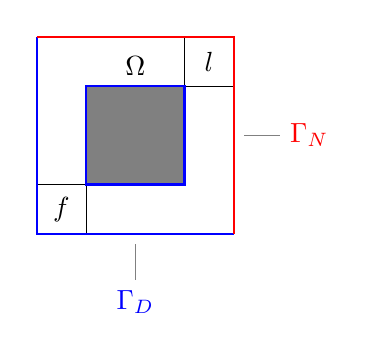
\begin{tikzpicture}[x=2.5cm,y=2.5cm]
    \node(n1) at (0,0){};
    \node(n2) at (1,0){};
    \node(n3) at (1,1){};
    \node(n4) at (0,1){};

    \node(n5) at (0.25,0.25){};
    \node(n6) at (0.75,0.25){};
    \node(n7) at (0.75,0.75){};
    \node(n8) at (0.25,0.75){};



    \draw (n1) rectangle (n5) node[pos=0.5] {$f$};
    \draw (n7) rectangle (n3) node[pos=0.5] {$l$};

    \draw[color=blue, thick, fill=gray] (n5) rectangle (n7);


    \draw[color=blue, thick] (n4.center) -- (n1.center) -- (n2.center) node[pos=0.5,pin={-90: $\Gamma_{D}$}]{};
    \draw[color=red, thick] (n4.center)--  (n3.center) -- node[pos=0.5,pin={0: $\Gamma_{N}$}]{} (n2.center);


    \node(omega) at (0.5,0.85){$\Omega$};

  \end{tikzpicture}
  \caption{Computational domain for Helmholtz Goal-Oriented Problem.\label{fig:HelmGOA}}
\end{figure}

\noindent In this case, we set the 2D-Laplace bilinear form as the form $\hat{b}$ to calculate the error estimator. \Cref{fig:resultsHelm2DGOAhem} shows the results for Helmholtz Goal-Oriented problem.
%
\subsection{Convection-Dominated Goal-Oriented Problem}
Let us consider the following Convection-Dominated Goal-Oriented problem.
\begin{var_for}
  Find $u$ such that,
  \begin{equation}
    \begin{cases}
      - \Delta u +b \cdot u= f & \text{ in } \Omega,       \\
      u=0                      & \text{ on } {\Gamma_{D}},
    \end{cases}
  \end{equation}
\end{var_for}
\noindent where $\vec{b} = (y,\frac{1}{2}-x)^{\textrm{T}}$ and $\Omega=(0,1)^{2}\symbol{92} (\frac{1}{3},\frac{2}{3})^{2}$. We set $\hat{b}(\cdot,\cdot)= \scalar{\grad \cdot}{\grad \cdot}_{L^{2}(\Omega)}$. The load function $f$ is chosen so that the exact solution $u$ is of the form $u = \sin(3 \pi x) \sin(3 \pi y) (2((x-0.1)^2 + (y-0.1))^2+10^{-3})^{-1}$. The \ac{QoI} is $l(\phi)=\int_{\Omega} 500 \exp (-500((x-0.9)^2 +(y-0.675)^2))\phi$, $\forall \phi \in \H$. The boundary conditions are illustrated in \Cref{fig:SPGOA}.

\begin{figure}
  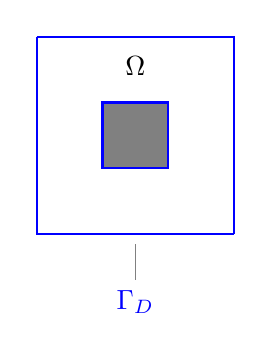
\begin{tikzpicture}[x=2.5cm,y=2.5cm]
    \node(n1) at (0,0){};
    \node(n2) at (1,0){};
    \node(n3) at (1,1){};
    \node(n4) at (0,1){};

    \node(n5) at (1/3,1/3){};
    \node(n7) at (2/3,2/3){};

    \draw[color=blue, thick, fill=gray] (n5) rectangle (n7);

    \draw[color=blue, thick] (n4.center) -- (n1.center) -- (n2.center) node[pos=0.5,pin={-90: $\Gamma_{D}$}]{};
    \draw[color=blue, thick] (n4.center)--  (n3.center) --  (n2.center);

    \node(omega) at (0.5,0.85){$\Omega$};

  \end{tikzpicture}
  \caption{Computational domain for Convection-Dominated Goal-Oriented Problem.\label{fig:SPGOA}}
\end{figure}

\noindent To reach $4.62 \cdot10^{-7} \%$ of error, our algorithm needs 21616 \acp{dof} and 13 iterations whereas the algorithm of \cite{holstpollock2016} require 18 iterations for delivering  around $1 \cdot10^{-2} \%$ of error. \Cref{fig:resultsSP2DGOA} shows the results for Convection-Dominated Goal-Oriented problem.

